\documentclass{article}
\usepackage[x11names]{xcolor}
\usepackage{amsmath}
\usepackage{graphicx}
\usepackage{amssymb}
\begin{document}
\textbf{fatgraph name: C5}
\definecolor{c0}{rgb}{0.5529411764705883, 0.8274509803921568, 0.7803921568627451}
\definecolor{c1}{rgb}{1.0, 1.0, 0.7019607843137254}
\definecolor{c2}{rgb}{0.7450980392156863, 0.7294117647058823, 0.8549019607843137}
\definecolor{c3}{rgb}{0.984313725490196, 0.5019607843137255, 0.4470588235294118}
\definecolor{c4}{rgb}{0.5019607843137255, 0.6941176470588235, 0.8274509803921568}
\definecolor{c5}{rgb}{0.9921568627450981, 0.7058823529411765, 0.3843137254901961}
\definecolor{c6}{rgb}{0.7019607843137254, 0.8705882352941177, 0.4117647058823529}
\definecolor{c7}{rgb}{0.9882352941176471, 0.803921568627451, 0.8980392156862745}
\definecolor{c8}{rgb}{0.8509803921568627, 0.8509803921568627, 0.8509803921568627}
\definecolor{c9}{rgb}{0.7372549019607844, 0.5019607843137255, 0.7411764705882353}
\definecolor{c10}{rgb}{0.8, 0.9215686274509803, 0.7725490196078432}
\definecolor{c11}{rgb}{1.0, 0.9294117647058824, 0.43529411764705883}
\begin{center}
\begin{figure}[h]
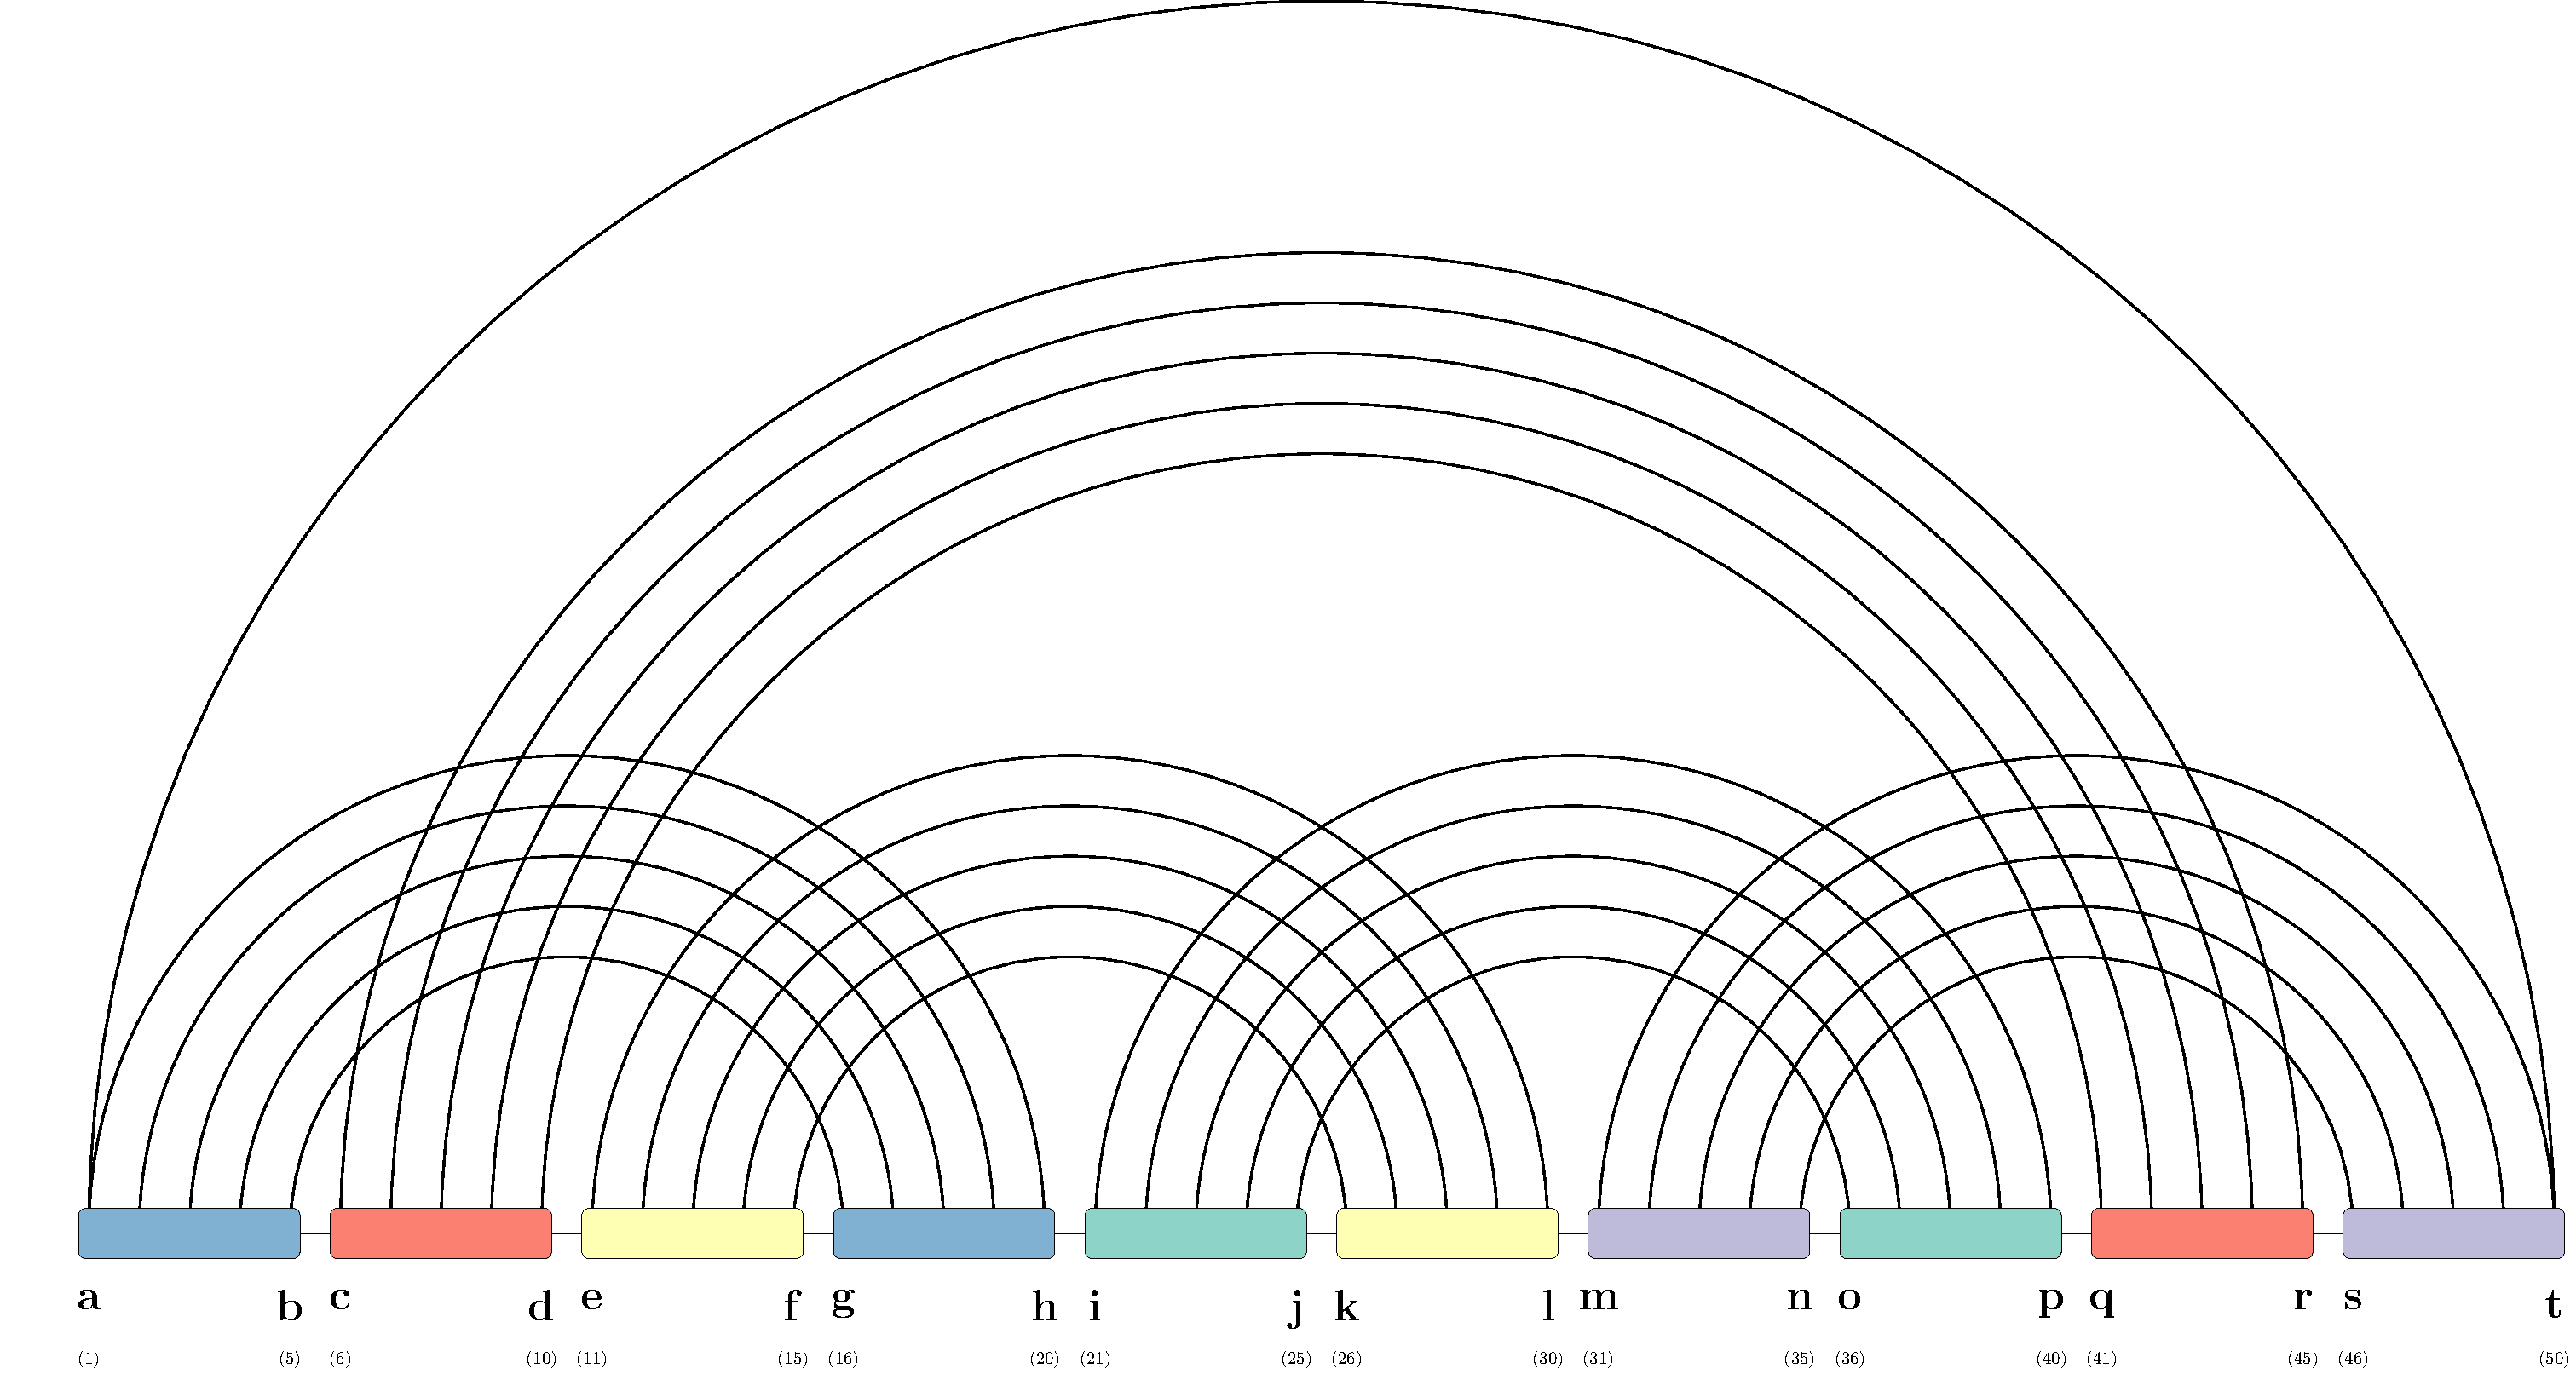
\includegraphics[width=\textwidth]{results/colored_dbn/colored_dbn_C5.pdf}
\end{figure}
\end{center}
first and last anchors, already given: $ a , t $
$$ A =\min_{ m,n,r } \left( B[r,n,m,a]+M[r,t,n,m]\right) $$
$$ B\left[ a,m,n,r \right] =\min_{ l } \left( C[r,n,l,a]\right) $$
$$ C\left[ a,l,n,r \right] =\min_{ h,k,p } \left( \colorbox{c4}{$D$}[a,h\mid r,p,l,k]+J[n,a,k,h,p]\right) $$
$$ \colorbox{c4}{$D$}' \left[a,h \mid  r,p,l,k \right] =  \min\begin{cases}\colorbox{c4}{$D$}'[ a , h-1\mid r,p,l,k ], &\text{if } h-1 ,\notin\{ a , r,p,l,k \} \\\colorbox{c4}{$D$}[ a+1 , h-1\mid r,p,l,k ]+\Delta G(a,h) &\text{if } \{ a+1 , h-1 \}\cap \{ r,p,l,k \}=\emptyset\end{cases}$$
$$ \colorbox{c4}{$D$} \left[a,h \mid  r,p,l,k \right] =  \min\begin{cases}\colorbox{c4}{$D$}[ a+1 , h\mid r,p,l,k ], &\text{if } a+1 \notin\{ h , r,p,l,k \} \\\colorbox{c4}{$D$}'[ a , h-1\mid r,p,l,k ], &\text{if } h-1 ,\notin\{ a , r,p,l,k \} \\\colorbox{c4}{$D$}[ a+1 , h-1\mid r,p,l,k ]+\Delta G(a,h) &\text{if } \{ a+1 , h-1 \}\cap \{ r,p,l,k \}=\emptyset,\\E[h,k,r,p,l,a]\end{cases}$$
$$ E\left[ b,g,k,l,p,r \right] =\min_{ e } \left( F[r,p,b,e]+I[k,e,g,l,b]\right) $$
$$ F\left[ b,e,p,r \right] =\min_{ c } \left( G[r,p,c,e]\right) $$
$$ G\left[ c,e,p,r \right] =\min_{ q } \left( H[r,c,e,q]\right) $$
$$ H\left[ c,e,q,r \right] =\min_{ d } \left( \colorbox{c3}{$C_{\boxtimes}$}[c,d,q,r]\right) $$
$$ I\left[ b,e,g,k,l \right] =\min_{ f } \left( \colorbox{c1}{$C_{\boxtimes}$}[e,f,k,l]\right) $$
$$ J\left[ a,h,k,n,p \right] =\min_{ i } \left( K[n,i,p,k]\right) $$
$$ K\left[ i,k,n,p \right] =\min_{ o } \left( L[p,o,i,k]\right) $$
$$ L\left[ i,k,o,p \right] =\min_{ j } \left( \colorbox{c0}{$C_{\boxtimes}$}[i,j,o,p]\right) $$
$$ M\left[ m,n,r,t \right] =\min_{ s } \left( \colorbox{c2}{$C_{\boxtimes}$}[m,n,s,t]\right) $$
\end{document}
